\section{A shared activity: poking}

A robot equipped with an arm and an active vision head was given a
simple ``poking'' behavior, whereby it selected objects in its
environment and struck them~\citep{fitzpatrick02towards}.
Since the robot had a limited reach,
this activity required the cooperation of a human
companion to bring the robot interesting objects to poke.
The behavior could also be preempted by the companion; when the robot
fixated an object and was about to reach for it, the companion
could choose to poke the object instead, in which case the robot
would refrain from acting.

This choice of activity has many benefits.  
%
{\em (i)}
The motion signature
generated by the impact of the arm with a rigid object greatly
simplifies segmenting that object from its background, and obtaining a
reasonable estimate of its boundary (see
Figure~\ref{fig:separate-simple}).  
This ``active segmentation''
procedure is key to automatically acquiring training data of
sufficient quality to support the many forms of learning described in
the remainder of this paper.
%
{\em (ii)}
The poking activity also leads to object-specific consequences, since
different objects respond to poking in different ways.  For example,
a toy car will tend to roll forward, while a bottle will roll along its
side.
%
{\em (iii)}
The basic operation involved, striking objects, can be performed
by either the robot or its human companion, creating a
controlled point of 
comparison between robot and human action.


%Get lots of object segmentations, tracked motion.  
%Cluster them.  Now can differentiate between objects,
%can see how they respond to poking individually.
%
%At this point can support basic mimicry (figures?).



\begin{figure}[bt]
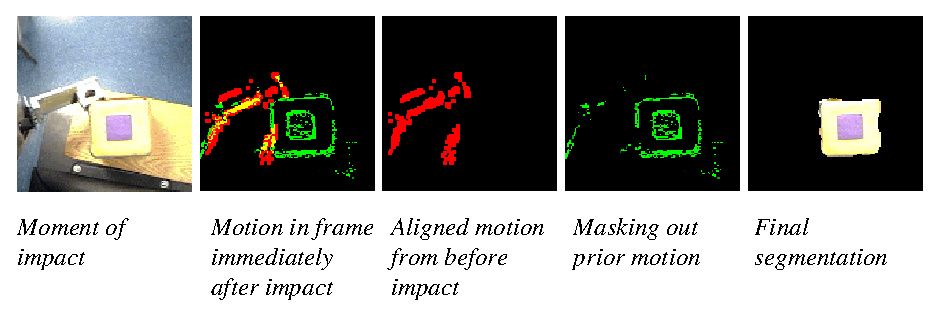
\includegraphics[width=\columnwidth]{fig-separate-simple}
\caption
{
\label{fig:separate-simple}
%
Active segmentation.  The robot arm is deliberately driven
to collide with an object.
 The
apparent motion after contact, when masked by the motion before
contact, identifies a seed foreground (object) region.  Such motion
will generally contain fragments of the arm and environmental motion
that escaped masking.  Motion present before contact is used to
identify background (non-object) regions.  
An optimal object region is computed from the foreground and
background information using graph cuts~\citep{boykov01experimental,
fitzpatrick03first}.
%
%This prevents the region
%assigned to the object motion from growing to include these fragments.
%The largest connected region, with a minor post-processing clean-up,
%is taken as the official segmentation of the object.
%
}
\end{figure}

